\chapter{Implementacija i korisničko sučelje}
		
		
		\section{Korištene tehnologije i alati}
		
			 U svrhu ovog projekta korištene su sljedeće tehnologije i alati: Django i Bootstrap web programski okviri, sustav za upravljanje bazom podataka PostGreSQL, program pgAdmin, jezici HTML, CSS i JavaScript te biblioteku jQuery. \\
			 
			 
			 {Za pisanje backenda korišten je Django, web programski okvir utemeljen na jeziku Python. Preuzeti se može na ovoj  \href{https://www.djangoproject.com/}{\textbf{poveznici}}.
			 	
			 Baza podataka ostvarena je kroz sustav \href{https://www.postgresql.org/}{\textbf{PostGreSQL}} te uz pomoć programa \href{https://www.pgadmin.org/}{\textbf{pgAdmin}}.
			 
			 Frontend dio ostvaren je kroz korištenje standardnih jezika \href{https://www.w3schools.com/html/}{\textbf{HTML}},\href{https://www.w3schools.com/css/}{\textbf{CSS}} te \href{https://www.w3schools.com/js/DEFAULT.asp}{\textbf{JavaScript}}. Linkovi vode na stranice gdje se o njima može više saznati. 
			 
			 Uz navedene jezike korišteni su i programski okvir \href{https://getbootstrap.com/}{\textbf{Bootstrap}} pomoću kojeg su dobivene neke napredne funkcionalnosti frontenda te biblioteke \href{https://jquery.com/}{\textbf{jQuery}}.
			
			
			\eject 
		
	
		\section{Ispitivanje programskog rješenja}
			
			
			Ispitivanje se provodilo ručno. Kao temelj za ispitivanje koristili su se obrasci uporabe. Osim preciznog praćenja obrazaca također smo i nasumično navigirali po stranici u slučaju da negdje postoje greške u kodu (bugovi). Iako smo provjerili cijeli sustav radi pojednostavljenja u dokumentaciji prikazujemo samo 6 ispitnih slučajeva. Ispitali smo: UC2, UC3, UC10, UC18, UC20, UC24
			\\
			\\ 
			\textbf{Ispitni slučaj 1: Detaljan pregled priča}
			\\
			\textbf{Ulaz}
			\\
			\indent 1. Pritisak kursorom na određenu priču
			\\
			\textbf{Očekivani rezultat}
			\\
			\indent 1. Preusmjeravanje na stranicu odabrane priče
			\\
			\textbf{Rezultat}
			\\
			\indent Očekivani rezultat je zadovoljen te smo preusmjereni na stranicu za detaljan pregled priče koje smo odabrali. Slučaj je testiran i kao prijavljen korisnik i kao gost. Aplikacija je prošla test.
			\\ \\
			\begin{figure}[H]
				\centering
				\includegraphics[scale=0.34]{"slike/test1"}
				\caption{Rezultat ispitnog slučaja 1}
				\label{fig:rezultat-ispitnog-slucaja-1}
			\end{figure}
			
			\noindent \textbf{Ispitni slučaj 2: Komentiranje priče}
			\\
			\textbf{Ulaz}
			\\
			\indent 1. Navigacija do detaljnog pregleda priče \\
			\indent 2. Upisivanje samog komentara u predviđeno mjesto \\
			\indent 3. Pritisak gumba "Objavi"
			\\
			\textbf{Očekivani rezultat}
			\\
			\indent 1. Spremanje komentara u bazu za kasniji prikaz na stranici priče \\
			\indent 2. Osvježavanje stranice
			\\
			\textbf{Rezultat}
			\\
			\indent Očekivani rezultat je zadovoljen te se stranica osvježila te vidimo komentar koji smo ostavili. Komentar smo uspješno ostavili i kao gost i kao prijavljeni korisnik. Aplikacija je prošla test.
			\\ \\
			\begin{figure}[H]
				\centering
				\includegraphics[scale=0.34]{"slike/test2"}
				\caption{Rezultat ispitnog slučaja 2}
				\label{fig:rezultat-ispitnog-slucaja-2}
			\end{figure}
			
			\noindent \textbf{Ispitni slučaj 3: Predlaganje priče administratoru}
			\\
			\textbf{Ulaz}
			\\
			\indent 1. Navigacija stranice za prijedlog priče \\
			\indent 2. Odabir medije, naslova zahtjeva i naslova priče \\
			\indent 3. Pritisak gumba "Predloži priču"
			\\
			\textbf{Očekivani rezultat}
			\\
			\indent 1. Spremanje prijedloga priče u bazu \\
			\indent 2. Preusmjeravanje na stranicu sandučića
			\\
			\textbf{Rezultat}
			\\
			\indent Očekivani rezultat je zadovoljen. Preusmjereni smo na stranicu sandučića na kojoj vidimo još neobrađen zahtjev naše priče. Aplikacija je prošla test.
			\\ \\
			\begin{figure}[H]
				\centering
				\includegraphics[scale=0.34]{"slike/test3"}
				\caption{Rezultat ispitnog slučaja 3}
				\label{fig:rezultat-ispitnog-slucaja-3}
			\end{figure}
			
			\noindent \textbf{Ispitni slučaj 4: Pregled košarice}
			\\
			\textbf{Ulaz}
			\\
			\indent 1. Pritisak na gumb "Košarica" \\
			\textbf{Očekivani rezultat}
			\\
			\indent 1. Prikaz sadržaja u košarici, ukupne cijene te gumba za dovršavanje narudžbe. \\
			\textbf{Rezultat}
			\\
			\indent Očekivani rezultat je zadovoljen. Pritiskom na gumb košarica otvora se prikaz već navedenog sadržaja. Aplikacija je prošla test.
			\\ \\
			\begin{figure}[H]
				\centering
				\includegraphics[scale=0.34]{"slike/test4"}
				\caption{Rezultat ispitnog slučaja 4}
				\label{fig:rezultat-ispitnog-slucaja-4}
			\end{figure}
			
			\noindent \textbf{Ispitni slučaj 5: Promjena profilne slike}
			\\
			\textbf{Ulaz}
			\\
			\indent 1. Navigacija do stranice profila \\
			\indent 2. Odabir datoteke na računalu \\
			\indent 3. Pritisak gumba "Promijeni profilnu sliku" \\
			\textbf{Očekivani rezultat}
			\\
			\indent 1. Osvježavanje trenutne stranice na kojoj vidimo da je profilna slika promijenjena \\
			\textbf{Rezultat}
			\\
			\indent Očekivani rezultat nije zadovoljen. Namjerno nije odabrana nijedna slika, a gumb je svejedno pritisnut. Stranica se osvježila te profilna slika nije ažurirana.
			\\ \\
			\begin{figure}[H]
				\centering
				\includegraphics[scale=0.34]{"slike/test5"}
				\caption{Rezultat ispitnog slučaja 5}
				\label{fig:rezultat-ispitnog-slucaja-5}
			\end{figure}
			
			\noindent \textbf{Ispitni slučaj 6: Pregled registriranih korisnika}
			\\
			\textbf{Ulaz}
			\\
			\indent 1. Pritisak na ime korisnika bilo gdje na stranici \\
			\textbf{Očekivani rezultat}
			\\
			\indent 1. Prikaz profila odabranog korisnika. \\
			\textbf{Rezultat}
			\\
			\indent Očekivani rezultat je zadovoljen. Pritiskom na korisničko ime u komentarima preusmjereni smo na pregled profila odabranog korisnika. Aplikacija je prošla test.
			\\ \\
			\begin{figure}[H]
				\centering
				\includegraphics[scale=0.34]{"slike/test6"}
				\caption{Rezultat ispitnog slučaja 6}
				\label{fig:rezultat-ispitnog-slucaja-6}
			\end{figure}
			
			
			\subsection{Ispitivanje sustava}
			
			 \textit{Potrebno je provesti i opisati ispitivanje sustava koristeći radni okvir Selenium\footnote{\url{https://www.seleniumhq.org/}}. Razraditi \textbf{minimalno 4 ispitna slučaja} u kojima će se ispitati redovni slučajevi, rubni uvjeti te poziv funkcionalnosti koja nije implementirana/izaziva pogrešku kako bi se vidjelo na koji način sustav reagira kada nešto nije u potpunosti ostvareno. Ispitni slučaj se treba sastojati od ulaza (npr. korisničko ime i lozinka), očekivanog izlaza ili rezultata, koraka ispitivanja i dobivenog izlaza ili rezultata.\\ }
			 
			 \textit{Izradu ispitnih slučajeva pomoću radnog okvira Selenium moguće je provesti pomoću jednog od sljedeća dva alata:}
			 \begin{itemize}
			 	\item \textit{dodatak za preglednik \textbf{Selenium IDE} - snimanje korisnikovih akcija radi automatskog ponavljanja ispita	}
			 	\item \textit{\textbf{Selenium WebDriver} - podrška za pisanje ispita u jezicima Java, C\#, PHP koristeći posebno programsko sučelje.}
			 \end{itemize}
		 	\textit{Detalji o korištenju alata Selenium bit će prikazani na posebnom predavanju tijekom semestra.}
			
			\eject 
		
		
		\section{Dijagram razmještaja}
			
			Sustav je baziran na arhitekturi "klijent-poslužitelj". Koristimo HTTP za komunikaciju između korisnikovog uređaja i poslužitelja. Za posluživanje koristimo Heroku koji nudi platformu kao uslugu u oblaku. Heroku se sam brine o portovima, operativnim sustavima i okolinama poslužitelja pa nisu prikazani u dijagramu.
			
			\begin{figure}[!h]
				\centering
				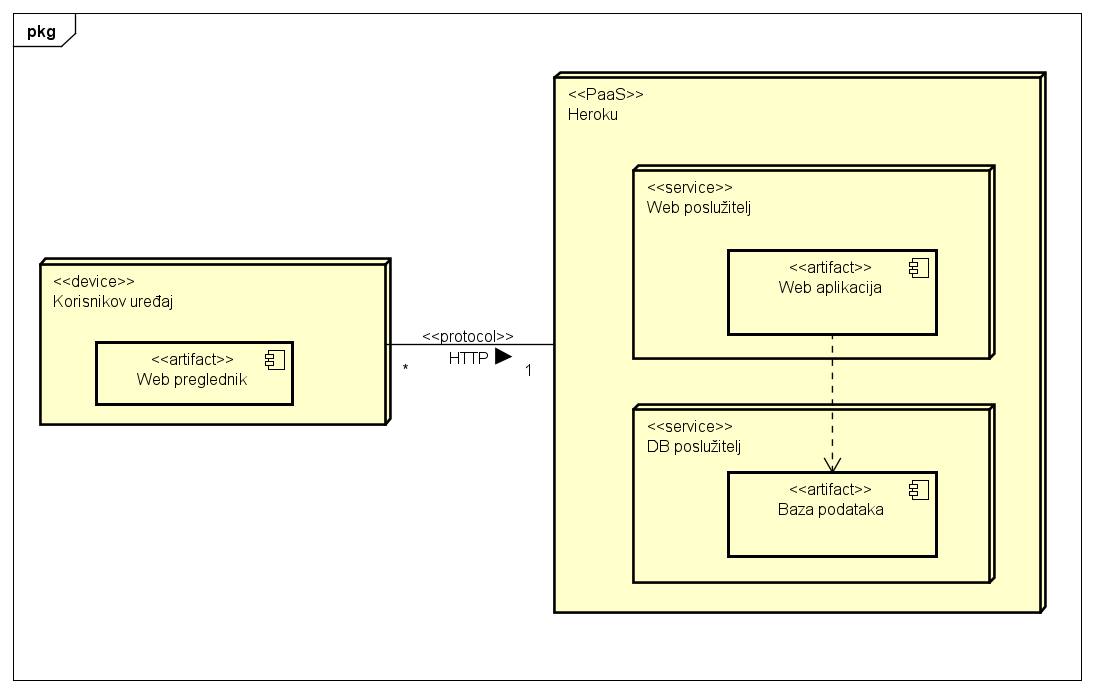
\includegraphics[width=1\linewidth]{slike/Dijagram_razmjestaja}
				\caption{Dijagram razmještaja}
				\label{fig:dijagramrazmjestaja}
			\end{figure}
			\eject
			
			\eject 
		
		\section{Upute za puštanje u pogon}
			\textbf{Instalacija Heroku poslužitelja}\\
			\\
			Potrebno je imati lokalno instalirani python verzije 3.8
			zajedno s najnovijom verzijom Django-a, najnoviju verziju Postgres-a, Git te besplatni Heroku račun.
			Potrebno je preuzeti Heroku Command Line Interface (CLI) koji je dostupan na https://cli-assets.heroku.com/heroku-x64.exe.
			Nakon toga potrebno je u Windows Command Prompt-u (cmd.exe) pokrenuti
			naredbu \verb|heroku login| koja će u zasebnom prozoru preglednika prikazati stranicu za login. \\
			\\
			\textbf{Konfiguracija aplikacije za Heroku}\\
			\\
			Kako bi se Heroku web aplikacija dobro konfigurirala potrebno je u
			Django server dodati 3 datoteke: \\
			1) requirements.txt s \\
			"Django==3.1.3 \\
			gunicorn==20.0.4 \\
			psycopg2-binary==2.8.6 \\
			pytz==2020.4 \\
			sqlparse==0.4.1 \\
			asgiref==3.3.0 \\
			dj-database-url==0.5.0 \\
			whitenoise==5.2.0 \\
			boto3==1.16.51 \\
			botocore==1.19.51 \\
			django-storages==1.11.1 \\
			jmespath==0.10.0 \\
			python-dateutil==2.8.1 \\
			s3transfer==0.3.3 \\
			six==1.15.0 \\
			urllib3==1.26.2" \\
			\\
			2) Procfile (bitno: Datoteka nema ekstenziju) s \\
			"web: gunicorn WeTried.wsgi --log-file -"
			\\
			3) runtime.txt s \\
			"python-3.8.6" \\
			\\
			\textbf{Stvaranje Heroku web aplikacije}\\
			\\
			Potrebno je imati lokalni git repozitorij koji se može stvoriti naredbom
			\verb|git init|.
			Pokretanjem naredbe 
			\verb|heroku create <name>| (naš name glasi "maketashop")
			stvara se heroku aplikacija i automatski se povezuje s lokalnim git repozitorijem.
			Nakon stvaranja aplikacije potrebno je dostaviti sam server pomoću naredbe \verb|git push heroku master|. Ako proces završi bez grešaka aplikacija je uspješno puštena u pogon, ostalo je samo povezati bazu s Djangom.
			\\
			\\
			\textbf{Konfiguriranje baze podataka}\\
			\\
			Heroku sam po sebi pri stvaranju python web aplikacije stvori addon
			postgresql tako da je potrebno samo u settings.py dodati \\
			\verb|"DATABASE_URL = <url>"| (url koji je generirao heroku) \\
			"DATABASES = {
				'default': dj\_database\_url.config(default=DATABASE\_URL)
			}"
			i \\
			"ALLOWED\_HOSTS = ['maketashop.herokuapp.com']". \\
			Nemojte zaboraviti maknuti konfiguraciju za korištenje lokalne baze podataka.
			
			\eject 